\section{Capacity commitment on five continents}\label{sec:global}

\subsection{A global panel of grid areas}

We assemble public hourly demand data for 125 grid areas on five continents (Table~\ref{tab:globaldata}).
\emph{North America} is the 46 U.S.\ balancing authorities of Section~\ref{sec:app} (EIA Form~930, 2019--2026), the only systems whose operators' day-ahead forecasts are in the data; elsewhere the reference rule is a model forecast (Section~\ref{sec:globalcand}).
\emph{Europe} contributes 33 national systems from Energy-Charts \citep{EnergyCharts}, including cross-border flows, and \emph{Oceania} the five regions of Australia's National Electricity Market \citep{AEMO}, both 2018--2026.
\emph{Asia} contributes 31 Chinese provinces for 2018 \citep{ChinaLoad2023}, four Taiwanese grid areas for 2018 to mid-2022 \citep{TaiwanLoad2023} and five Thai regions for 2023--2024 \citep{ThaiLoad2025}; \emph{Africa} is Algeria (Sonelgaz), 2018 to January 2020 \citep{AlgeriaLoad2023}.
All series are converted to hourly UTC, cleaned as in Section~\ref{sec:app}, and placed on a common calendar from 1 January 2018 to 26 September 2026.
The average demands sum to 1.66\,TW, which is not demand served at any one time because areas are observed in different periods.
The panel is deliberately unbalanced: several Asian and African systems have only one or two years of data, as is typical of emerging economies, and an area contributes only on days with data.
Other large systems (South Africa, India, Japan, South Korea) could not be retrieved (Section~\ref{sec:conclusion}).

\begin{table}[t]
\centering
\caption{The global panel.}\label{tab:globaldata}
\small
\begin{tabular}{@{}llrcr@{}}
\toprule
Continent & Systems & Areas & Period & Mean demand \\
\midrule
North America & U.S.\ balancing authorities (EIA-930) & 46 & 2019--2026 & 455\,GW \\
Europe & National systems (Energy-Charts) & 33 & 2018--2026 & 339\,GW \\
Oceania & NEM regions, Australia (AEMO) & 5 & 2018--2026 & 21\,GW \\
Asia & China (31 provinces) & 31 & 2018 & \multirow{3}{*}{839\,GW} \\
 & Taiwan (4 grid areas) & 4 & 2018--2022 & \\
 & Thailand (5 regions) & 5 & 2023--2024 & \\
Africa & Algeria (Sonelgaz) & 1 & 2018--2020 & 7\,GW \\
\midrule
Total & & 125 & 2018--2026 & 1.66\,TW \\
\bottomrule
\end{tabular}
\end{table}

\begin{figure}[t]
\centering
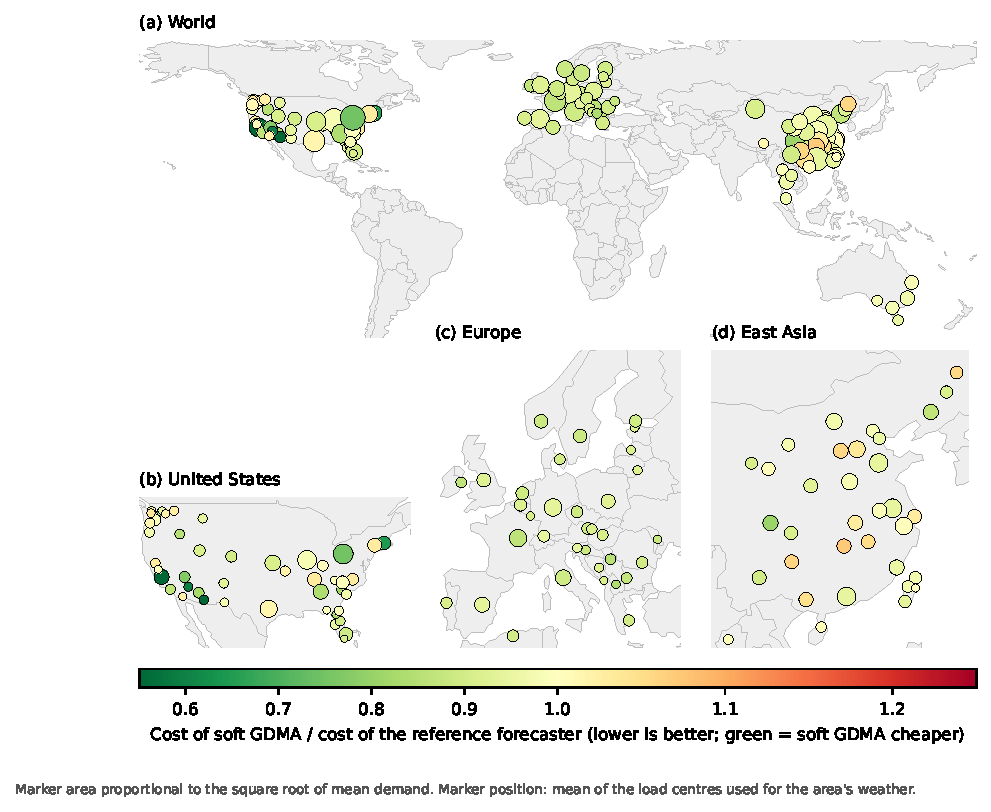
\includegraphics[width=0.95\textwidth]{figures/fig_map_gain.pdf}
\caption{Where soft GDMA saves cost. Each marker is one of the 125 grid areas, coloured by the cost of soft GDMA relative to the reference forecaster ($W=28$; lower is better, values below 1 mean a lower cost). Marker size shows mean demand.}\label{fig:mapgain}
\end{figure}

Soft GDMA has a lower cost than the reference in every European area (0.84--0.95); the largest gains are in three western U.S.\ balancing authorities (Tucson, the California ISO and the Lower Colorado area, 0.45--0.59), and 25 of the 125 areas, 13 of them in China, have a higher cost (Figure~\ref{fig:mapgain}).

\subsection{Candidates, costs and competitors}\label{sec:globalcand}

Every area receives eleven candidate forecasts: the seven of Section~\ref{sec:app}; a zero-shot forecast from the pretrained foundation model Chronos-Bolt (small; \citealp{Ansari2024chronos}), which takes the 28 days of demand known at decision time, forecasts 48 hours and contributes the last 24; and three weather-aware global LightGBM models.
Chronos was pretrained on public series including electricity load, so some of our data may be in its corpus.
Outside the United States candidate~0, the \emph{reference forecaster}, is the global LightGBM forecast, a strong rule distinct from the best single candidate.
The temperature model adds to the LightGBM features the operating day's hourly, mean, minimum and maximum 2-m temperature, heating and cooling degrees (base 18\,$^\circ$C) and the previous day's mean, from NASA POWER \citep{NASAPOWER} averaged over one to five load centres per area (169 locations).
Realised temperature would be an \emph{ex post} forecast in the terminology of \citet{HongFan2016}, so the weather models use \emph{archived day-ahead forecasts} of NOAA's Global Forecast System \citep{GFSarchive}: for day $d$, the 00~UTC run of day $d-1$ at lead times of 24 to 48 hours, interpolated to the load centres and to hourly resolution (the previous day's temperature is the forecast for day $d-1$ issued on day $d-2$).
The run is available at about 04--05~UTC, before a 10:00-local gate closure in the Americas, Europe and Algeria but after it in East Asia and Australia, so only the first group uses weather forecasts.
The archive starts in January 2021; before then the weather models use their other features.
The GFS forecasts have a root-mean-squared error of 2.3\,$^\circ$C against realised temperatures (1.9 in Europe, 2.2 in North America, 2.7 in Asia); a version with realised temperatures is an upper bound.
The \emph{multi-variable model} adds, from the same GFS runs, forecast 2-m relative humidity, 10-m wind speed and downward short-wave radiation, and from the GEFSv12 ensemble \citep{GEFSv12,GEFSarchive} the standard deviation of 2-m temperature at 0.5 degrees (from October 2020).
The third weather candidate uses this spread for the commitment margin: it multiplies the multi-variable model's quantile margin by the ratio of the day's spread to its mean over the previous 28 days, clipped to $[0.5,3]$ (\emph{ensemble margin}).
The rule was motivated by Winter Storm Elliott and uses a raw, uncalibrated spread from a single archive, so it is exploratory; its constants were set once, untuned.
The spread says little about the error on an average day (rank correlation 0.04 across area-days, 0.08 within areas) but is large in unusual weather.
Mean absolute errors, scaled by mean demand, are 3.5\% for the temperature and multi-variable models (also with exact temperatures), 3.6\% for LightGBM, 3.8\% for Chronos, 4.5\% for the official/LightGBM candidate and 6--8\% for the naive rules.

Critical ratios follow the flexibility rule of Section~\ref{sec:app} wherever interchange is measured (the United States, 31 European countries, and Taiwan, an island grid with zero flexibility); the rest receive the midpoint $\tau=0.875$.
A common $\tau$ gives the same ranking (Section~\ref{sec:robust}, Table~\ref{tab:globaltau}).

Beyond the benchmarks of Section~\ref{sec:app}, we add a \emph{decision-focused neural gate}, a two-hidden-layer perceptron (NGPARAMS parameters with eleven candidates).
From features at the weekly origin (each candidate's decision cost and forecast error over the last 7 and 28 known days, the critical ratio, recent demand, data share, continent and season) it produces combination weights through a softmax, as in mixture-of-experts averaging \citep{Gong2026moe}.
It is trained end to end on the same smoothed newsvendor cost, on up to 52 recent weeks with fully observed outcomes, and re-trained every four weeks; the four most recent weeks serve for early stopping, and two initialisations are averaged.
It is untuned.
Unlike GDMA it lets weights vary continuously with conditions; like GDMA it uses only information available at decision time.

\subsection{Results}

\begin{table}[t]
\centering
\caption{Out-of-sample commitment cost on five continents ($W=28$ days, May 2018 to September 2026, eleven candidates including the three weather models), relative to the reference forecaster. Bold: lowest in the column. Stars: Diebold--Mariano test of equal daily cost against soft GDMA (Newey--West, 7 lags); $^{*}$, $^{**}$, $^{***}$: $p<0.10,0.05,0.01$. $^\dagger$: member of the 90\% model confidence set. Lower is better: values below 1 mean a lower cost than the benchmark.}\label{tab:global}
\footnotesize
\setlength{\tabcolsep}{4pt}
\begin{tabular}{@{}lcccccc@{}}
\toprule
Method & World & North America & Europe & Oceania & Asia & Africa \\
\midrule
Single best forecaster$^a$ & 1.000$^{***}$ & 1.000$^{***}$ & 1.000$^{***}$ & 1.000$^{***}$ & 1.000$^{***}$ & 1.000$^{***}$ \\
Equal weights & 1.252$^{***}$ & 1.383$^{***}$ & 1.144$^{***}$ & 1.000$^{***}$ & 1.135$^{***}$ & 1.022$^{***}$ \\
Best single (per area) & 0.863$^{***}$ & 0.843$^{***}$ & 0.889$^{***}$ & 0.815 & 0.891$^{***}$ & 0.872$^{***}$ \\
Pooled DF weights & 0.860$^{***}$ & 0.835$^{***}$ & 0.888$^{***}$ & 0.871$^{***}$ & 0.865$^{***}$ & 0.825$^{*}$ \\
Per-area DF weights & 0.829$^{***}$ & 0.799 & 0.860$^{***}$ & 0.798$^{***}$ & 0.879$^{***}$ & 0.830$^{**}$ \\
Shrinkage to pooled & 0.824$^{***}$ & \textbf{0.796} & 0.854$^{***}$ & 0.812 & 0.851$^{*}$ & 0.811 \\
Two-step $k$-means & 0.824$^{***}$ & 0.801$^{**}$ & 0.847$^{*}$ & 0.812 & 0.852$^{*}$ & 0.831$^{**}$ \\
Forecast-then-commit, per area & 0.912$^{*}$ & 0.927 & 0.870$^{***}$ & \textbf{0.796}$^{***}$ & 1.124 & 0.840 \\
Forecast-then-commit, grouped & 0.907 & 0.940 & 0.844 & 0.799$^{***}$ & 1.100 & 0.809 \\
Neural gate (deep MoE) & 0.916$^{***}$ & 0.944$^{***}$ & 0.882$^{***}$ & 0.798$^{***}$ & 0.985$^{***}$ & 0.848$^{***}$ \\
GDMA & 0.827$^{***}$ & 0.808$^{***}$ & 0.846$^{*}$ & 0.827$^{***}$ & 0.850$^{*}$ & 0.813 \\
\textbf{Soft GDMA} & 0.820 & 0.797 & 0.843 & 0.813 & 0.848 & \textbf{0.808} \\
Fair soft GDMA & \textbf{0.817}$^{***}$ & 0.798 & \textbf{0.836}$^{***}$ & 0.803$^{***}$ & \textbf{0.845} & 0.815$^{*}$ \\
\midrule
Grid areas & 125 & 46 & 33 & 5 & 40 & 1 \\
\bottomrule
\end{tabular}
\par\smallskip\footnotesize $^a$ The operator's official forecast where one is published (United States), otherwise the global LightGBM forecast.
\end{table}

Table~\ref{tab:global} shows that the main U.S.\ findings carry over to the world panel, with smaller savings.
Worldwide, soft GDMA lowers the commitment cost by 11.6\% relative to the reference forecaster and by 4.2 percentage points relative to the best single candidate; its fair variant lowers it by 11.9\%.
The 90\% model confidence set \citep{Hansen2011mcs} contains four methods (two-step clustering, GDMA, soft GDMA and fair soft GDMA); it excludes shrinkage towards pooled weights ($p=0.098$) and per-area weights only narrowly, and the neural gate, the quantile-regression combination and the best single candidate more clearly.
Within the set the differences are below 0.4\%; fair soft GDMA is the cheapest in total (0.881), significantly so against soft GDMA.
By continent a GDMA variant is cheapest in North America and Africa, the neural gate nominally in Europe and Oceania (0.896 and 0.964, against 0.897 and 0.972 for the best GDMA variant), and pooled weights in Asia (0.929 against 0.963--0.965), where most areas have little data.

Three comparisons stand out.
First, decision-focused combination on the simplex dominates forecast-then-commit and the unconstrained quantile-regression combination: combining forecasts for accuracy and adding a quantile margin saves only 1--3\% worldwide, and the quantile-regression combination costs more than the reference (1.016) because, with eleven collinear candidates and few weeks of data, freeing the weights from the simplex costs more in variance than it gains; both are poor in Asia.
Second, the neural gate is clearly worse than the simple decision-focused rules (0.956 against 0.884 worldwide), although competitive in Europe and Oceania; flexibility alone does not solve the problem, but an untuned gate says little about the best neural design.
Third, better candidates and better combination are complements.
On their own the temperature model costs 0.965 of the reference, the multi-variable model 0.960, its ensemble-margin version 0.981, LightGBM 0.988 and the zero-shot foundation model 1.434, which must forecast two days ahead.
Adding the temperature model lowers the cost of soft GDMA from 0.906 to 0.892 and the two multi-variable candidates to 0.884 (Table~\ref{tab:specs}); with realised temperatures it is 0.876.
The method ranking is the same for every candidate set and similar across windows and critical ratios (Tables~\ref{tab:globalwindows} and~\ref{tab:globaltau}).

\begin{table}[t]
\centering
\caption{World commitment cost relative to the reference forecaster for four candidate sets ($W=28$): eight candidates without weather; nine with the temperature model fed archived GFS forecasts; eleven with, in addition, the multi-variable model and its ensemble-margin version (main specification); and nine with realised temperatures (upper bound). Lower is better: values below 1 mean a lower cost than the benchmark.}\label{tab:specs}
\footnotesize
\begin{tabular}{@{}lcc@{}}
\toprule
Method & No weather (8 candidates) & Weather, forecast error 2$^\circ$C (main) \\
\midrule
Single best forecaster$^a$ & 1.000 & 1.000 \\
Equal weights & 1.315 & 1.252 \\
Best single (per area) & 0.870 & 0.866 \\
Pooled DF weights & 0.872 & 0.861 \\
Per-area DF weights & 0.838 & 0.830 \\
Shrinkage to pooled & 0.833 & 0.824 \\
Two-step $k$-means & 0.832 & 0.824 \\
Forecast-then-commit, per area & 0.923 & 0.913 \\
Forecast-then-commit, grouped & 0.917 & 0.906 \\
Neural gate (deep MoE) & 0.918 & 0.916 \\
GDMA & 0.835 & 0.826 \\
\textbf{Soft GDMA} & 0.828 & 0.819 \\
Fair soft GDMA & -- & 0.816 \\
\bottomrule
\end{tabular}
\end{table}

\paragraph{Extreme events}
In the U.S.\ analysis (Table~\ref{tab:events}) the operators' own forecasts beat every combination during Winter Storm Elliott, the abrupt cold snap of 21--26 December 2022 \citep{FERCNERC2023}.
Over the six days soft GDMA has a 20.0\% higher cost than the official forecasts without weather candidates, 14.7\% with GFS temperature forecasts and 9.5\% with the multi-variable candidates, and 11.1\% with realised temperatures (Table~\ref{tab:elliott}); six days are too few to rank candidate sets.
Excluding the BA-days on which TVA and Duke shed load \citep{FERCNERC2023}, which understate demand, the excess is 8.4\%.
Only the multi-variable model with the ensemble margin beats the operators, at a 7\% lower cost (0.929), because the GEFS spread rose on 23 December, the costliest day, and widened the margin by a median factor of 1.4.
This is exploratory: the rule was designed after the gap was known and is evaluated on the event that motivated it; it is the most expensive weather candidate over the whole period (0.981), and the combination rules do not give it enough weight.
During Winter Storm Uri, soft GDMA has an 11--13\% lower cost than the operators in every candidate set, also excluding ERCOT's, SPP's and MISO's load-shed days.

\begin{table}[t]
\centering
\caption{Winter Storm Elliott (21--26 December 2022, 46 U.S.\ balancing authorities): commitment cost relative to the operators' official day-ahead forecasts, by candidate set ($W=28$), and in the main set without the BA-days on which load was shed. Lower is better: values below 1 mean a lower cost than the benchmark.}\label{tab:elliott}
\footnotesize
\setlength{\tabcolsep}{4pt}
\begin{tabular}{@{}lccccc@{}}
\toprule
 & \begin{tabular}[b]{@{}c@{}}No\\weather\end{tabular} & \begin{tabular}[b]{@{}c@{}}GFS\\temperature\end{tabular} & \begin{tabular}[b]{@{}c@{}}GFS/GEFS\\multi-variable\end{tabular} & \begin{tabular}[b]{@{}c@{}}Realised\\temperature\end{tabular} & \begin{tabular}[b]{@{}c@{}}Main set,\\no shed days\end{tabular} \\
\midrule
\multicolumn{6}{@{}l}{\emph{Combination rules}} \\
\textbf{Soft GDMA} & 1.080 & 1.075 & 1.034 & 1.057 & 1.012 \\
Fair soft GDMA & -- & 1.053 & 1.065 & 1.064 & 1.030 \\
GDMA & 1.101 & 1.055 & 1.043 & 1.055 & 1.003 \\
Two-step $k$-means & 1.106 & 1.039 & 1.070 & 1.118 & 1.034 \\
Shrinkage to pooled & 1.087 & 1.078 & 1.044 & 1.101 & 1.018 \\
Per-area DF weights & 1.088 & 1.093 & 1.046 & 1.120 & 1.038 \\
Pooled DF weights & 1.140 & 1.091 & 1.085 & 1.104 & 1.034 \\
Best single (per area) & 1.225 & 1.127 & 1.110 & 1.129 & 1.075 \\
Forecast-then-commit, grouped & 1.313 & 1.200 & 1.181 & 1.219 & 1.127 \\
\midrule
\multicolumn{6}{@{}l}{\emph{Weather candidates on their own}} \\
Temperature model & -- & -- & -- & -- & -- \\
Multi-variable model & -- & -- & -- & -- & -- \\
Multi-variable, ensemble margin & -- & -- & -- & -- & -- \\
\bottomrule
\end{tabular}
\end{table}

As a single storm is a weak basis, we also examine all extreme-temperature area-days, fixed beforehand as those with daily mean temperature below its 2.5\% or above its 97.5\% quantile (Table~\ref{tab:extremes}).
On cold days soft GDMA has a 12\% lower cost than the reference worldwide (90\% interval 0.83--0.93, block bootstrap over days) and on hot days 19\% lower (0.79--0.84); in the United States 10\% and 25\% lower.
Elliott is thus atypical: an abrupt cold snap with large forced outages, which weights cannot anticipate.

\begin{table}[t]
\centering
\caption{Commitment cost relative to the reference forecaster on extreme-temperature area-days ($W=28$): days on which an area's daily mean temperature is below its 2.5\% or above its 97.5\% quantile. Intervals: moving-block bootstrap over days (7-day blocks, 1,000 replications). Lower is better: values below 1 mean a lower cost than the benchmark.}\label{tab:extremes}
\footnotesize
\setlength{\tabcolsep}{4pt}
\begin{tabular}{@{}lcccc@{}}
\toprule
 & \begin{tabular}[b]{@{}c@{}}World\\cold\end{tabular} & \begin{tabular}[b]{@{}c@{}}World\\hot\end{tabular} & \begin{tabular}[b]{@{}c@{}}U.S.\\cold\end{tabular} & \begin{tabular}[b]{@{}c@{}}U.S.\\hot\end{tabular} \\
\midrule
Reference forecaster$^a$ & 1.000 & 1.000 & 1.000 & 1.000 \\
Equal weights & 1.151 & 0.919 & 1.323 & 0.885 \\
Best single (per area) & 0.877 & 0.789 & 0.941 & 0.751 \\
Pooled DF weights & 0.848 & 0.743 & 0.888 & 0.688 \\
Per-area DF weights & 0.804 & 0.736 & 0.832 & 0.689 \\
Shrinkage to pooled & 0.800 & 0.723 & 0.827 & 0.678 \\
Two-step $k$-means & 0.804 & 0.739 & 0.844 & 0.693 \\
Forecast-then-commit, per area & 1.004 & 0.803 & 1.163 & 0.756 \\
Forecast-then-commit, grouped & 0.982 & 0.766 & 1.169 & 0.712 \\
Neural gate (deep MoE) & 0.844 & 0.763 & 0.921 & 0.723 \\
GDMA & 0.815 & 0.736 & 0.860 & 0.693 \\
\textbf{Soft GDMA} & 0.803 & 0.728 & 0.841 & 0.684 \\
Fair soft GDMA & 0.804 & 0.730 & 0.851 & 0.686 \\
\midrule
Soft GDMA / reference, 90\% CI & [0.77, 0.84] & [0.70, 0.75] & [0.80, 0.89] & [0.65, 0.72] \\
Soft GDMA / best single, 90\% CI & [0.89, 0.94] & [0.90, 0.94] & [0.86, 0.93] & [0.88, 0.94] \\
Area-days & 9,624 & 9,623 & 3,542 & 3,540 \\
\bottomrule
\end{tabular}
\par\smallskip\footnotesize $^a$ As in Table~\ref{tab:global}.
\end{table}

\begin{figure}[t]
\centering
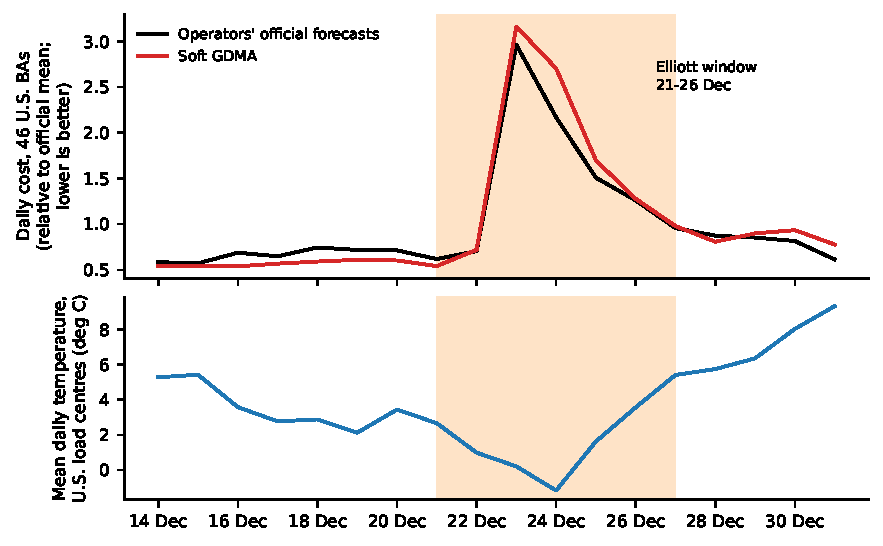
\includegraphics[width=0.8\textwidth]{figures/fig_elliott.pdf}
\caption{Winter Storm Elliott, 14--31 December 2022: daily commitment cost of the 46 U.S.\ balancing authorities (relative to the mean daily cost under the operators' forecasts; lower is better) and mean temperature of their load centres. Shaded: the FERC--NERC window.}\label{fig:elliott}
\end{figure}

\paragraph{Tail risk}
To see the tail, Table~\ref{tab:tail} reports the average of the costliest 5\% of days (CVaR$_{95}$) and the costliest week of the world's daily cost.
Soft GDMA's costliest week costs 16\% less than the reference's (0.840) and its CVaR$_{95}$ is 9.5\% lower (0.905), so its saving is not bought with a heavier tail.
Forecast-then-commit and quantile-regression rules fail in the tail: their CVaR$_{95}$ is 55--63\% higher and their costliest week nine times as costly, mostly in the first week of January 2019, when the 46 U.S.\ balancing authorities enter with a few days of data (more than twice as costly even without each area's first eight weeks).
With a scarcity-level critical ratio of 0.99 for every area, soft GDMA's total cost is 11\% lower (0.888), its CVaR$_{95}$ 8\% lower and its costliest week 10\% lower; forecast-then-commit and the quantile-regression combination cost more than the reference in total (1.18--1.53) and 14--15 times as much in their costliest week.
Equal weights have the lightest tail at this ratio (costliest week 0.66) but a higher total cost (1.071).

\begin{table}[t]
\centering
\caption{Tail risk of the world's daily commitment cost relative to the reference forecaster ($W=28$): total, average of the costliest 5\% of days (CVaR$_{95}$) and costliest week, for the calibrated critical ratios, without each area's first eight weeks, and with a scarcity-level critical ratio of 0.99 for every area. Lower is better: values below 1 mean a lower cost than the benchmark.}\label{tab:tail}
\scriptsize
\setlength{\tabcolsep}{2.5pt}
\begin{tabular}{@{}lcccccccc@{}}
\toprule
 & \multicolumn{3}{c}{Calibrated $\tau_i$ (main)} & \multicolumn{2}{c}{Without first} & \multicolumn{3}{c}{$\tau_i=0.99$ for every area} \\
 & & & & \multicolumn{2}{c}{8 weeks of each area} & & & \\
\cmidrule(lr){2-4}\cmidrule(lr){5-6}\cmidrule(lr){7-9}
Method & Total & \begin{tabular}[b]{@{}c@{}}CVaR$_{95}$\\daily\end{tabular} & \begin{tabular}[b]{@{}c@{}}Worst\\week\end{tabular} & \begin{tabular}[b]{@{}c@{}}CVaR$_{95}$\\daily\end{tabular} & \begin{tabular}[b]{@{}c@{}}Worst\\week\end{tabular} & Total & \begin{tabular}[b]{@{}c@{}}CVaR$_{95}$\\daily\end{tabular} & \begin{tabular}[b]{@{}c@{}}Worst\\week\end{tabular} \\
\midrule
Reference forecaster$^a$ & 1.000 & 1.000 & 1.000 & 1.000 & 1.000 & -- & -- & -- \\
Equal weights & 1.217 & 1.136 & 1.068 & 1.114 & 1.019 & -- & -- & -- \\
Best single (per area) & 0.923 & 0.981 & 0.946 & 0.971 & 0.905 & -- & -- & -- \\
Pooled DF weights & 0.902 & 0.914 & 0.919 & 0.901 & 0.830 & -- & -- & -- \\
Per-area DF weights & 0.895 & 0.920 & 0.829 & 0.908 & 0.845 & -- & -- & -- \\
Shrinkage to pooled & 0.888 & 0.902 & 0.845 & 0.893 & 0.805 & -- & -- & -- \\
Two-step $k$-means & 0.884 & 0.892 & 0.853 & 0.884 & 0.785 & -- & -- & -- \\
Quantile-regression comb. & 1.016 & 1.634 & 8.955 & 1.152 & 2.316 & -- & -- & -- \\
Forecast-then-commit, per area & 0.988 & 1.603 & 8.968 & 1.117 & 2.313 & -- & -- & -- \\
Forecast-then-commit, grouped & 0.966 & 1.554 & 8.995 & 1.067 & 2.274 & -- & -- & -- \\
Neural gate (deep MoE) & 0.956 & 0.943 & 0.996 & 0.859 & 0.794 & -- & -- & -- \\
GDMA & 0.884 & 0.902 & 0.866 & 0.893 & 0.804 & -- & -- & -- \\
\textbf{Soft GDMA} & 0.884 & 0.905 & 0.840 & 0.895 & 0.820 & -- & -- & -- \\
Fair soft GDMA & 0.881 & 0.898 & 0.848 & 0.888 & 0.826 & -- & -- & -- \\
\bottomrule
\end{tabular}
\end{table}

\paragraph{New and data-poor systems}
Fifty-two areas enter after the evaluation starts (the 46 U.S.\ balancing authorities in January 2019, the five Thai regions in January 2023, one European system) and have only a few weeks of history in their first eight weeks (Table~\ref{tab:entry}).
No combination does well then: all except the quantile-regression combination (0.976) cost more than the reference.
Pooled weights cost 61\% more, forecast-then-commit 39--40\% more, and the neural gate, whose features are not yet informative, 2.6 times as much.
Plain GDMA (1.053) and fair soft GDMA (1.058) are closest to the reference, followed by soft GDMA and the best single candidate (1.069, each); per-area weights and shrinkage cost 11\% more, and two-step clustering (1.170) more still because it clusters weights estimated from a handful of days.
The quantile-regression combination beats the reference for entering areas but not for established ones (1.016); we cannot explain this and the entry sample is small.
Where an official forecast exists, an operator should keep committing on it for a new unit's first weeks.

\begin{table}[t]
\centering
\caption{Commitment cost of areas entering the panel, relative to the reference forecaster ($W=28$, eleven candidates). Lower is better: values below 1 mean a lower cost than the benchmark.}\label{tab:entry}
\footnotesize
\begin{tabular}{@{}lcc@{}}
\toprule
Method & First 8 weeks after entry$^b$ & All other weeks \\
\midrule
Single best forecaster$^a$ & 1.000 & 1.000 \\
Equal weights & 2.120 & 1.307 \\
Best single (per area) & 0.994 & 0.869 \\
Pooled DF weights & 1.233 & 0.868 \\
Per-area DF weights & 0.991 & 0.836 \\
Shrinkage to pooled & 1.012 & 0.831 \\
Two-step $k$-means & 0.971 & 0.831 \\
Forecast-then-commit, per area & 1.037 & 0.922 \\
Forecast-then-commit, grouped & 1.283 & 0.914 \\
Neural gate (deep MoE) & 1.629 & 0.911 \\
GDMA & 1.039 & 0.833 \\
\textbf{Soft GDMA} & 0.978 & 0.827 \\
\midrule
Grid areas entering & 52 & \\
\bottomrule
\end{tabular}
\par\smallskip\footnotesize $^b$ The first eight weeks after an area has at least one day of data in the estimation window.
\end{table}

\paragraph{Segments across continents}
GDMA uses more than one segment in 89\% of weekly re-estimations (two in 20\%, three in 22\%, four in 21\%), much more than in the U.S.\ panel; soft GDMA shrinks towards the segment rule with an average $\kappa=0.39$.
Segments are not continents: among weeks with several segments, two systems on the same continent share one only 37--49\% of the time, European and African systems 52\%, and North American areas with European or Asian ones 19--21\%.
The segmentation fits differences in which forecasting systems work, notably whether an operator's own forecast is available and informative, which a planner could not specify in advance.

\subsection{Who benefits? A fairness audit}\label{sec:fairaudit}

\begin{table}[t]
\centering
\caption{Distribution of the benefits across the 125 grid areas ($W=28$, eleven candidates): percentiles of each area's cost relative to the reference forecaster, share of areas made worse off than under the reference and under their own best single candidate, median ratio in the worst-served continent, and cost ratios for data-rich and data-poor areas. Cost ratios and shares: lower is better.}\label{tab:fairness}
\scriptsize
\setlength{\tabcolsep}{3pt}
\begin{tabular}{@{}lccccccc@{}}
\toprule
 & \multicolumn{3}{c}{Per-area cost ratio} & Areas & Worst & Data-rich & Data-poor \\
\cmidrule(lr){2-4}
Method & P10 & Median & P90 & harmed & continent$^d$ & areas & areas$^e$ \\
\midrule
Single best forecaster$^a$ & 1.000 & 1.000 & 1.000 & 0.00 & 1.000 & 1.000 & 1.000 \\
Equal weights & 0.949 & 1.075 & 1.454 & 0.78 & 1.166 & 1.168 & 1.103 \\
Best single (per area) & 0.785 & 0.901 & 1.011 & 0.15 & 0.930 & 0.857 & 0.915 \\
Pooled DF weights & 0.785 & 0.883 & 1.009 & 0.13 & 0.891 & 0.853 & 0.862 \\
Per-area DF weights & 0.761 & 0.873 & 0.980 & 0.06 & 0.909 & 0.818 & 0.903 \\
Shrinkage to pooled & 0.763 & 0.860 & 0.969 & 0.05 & 0.882 & 0.816 & 0.863 \\
Two-step $k$-means & 0.773 & 0.859 & 0.973 & 0.05 & 0.881 & 0.816 & 0.863 \\
Forecast-then-commit, per area & 0.784 & 0.905 & 1.154 & 0.27 & 0.959 & 0.907 & 0.916 \\
Forecast-then-commit, grouped & 0.786 & 0.887 & 1.164 & 0.26 & 0.975 & 0.904 & 0.873 \\
Neural gate (deep MoE) & 0.791 & 0.916 & 1.135 & 0.32 & 1.041 & 0.903 & 1.036 \\
GDMA & 0.772 & 0.863 & 0.978 & 0.08 & 0.887 & 0.819 & 0.863 \\
\textbf{Soft GDMA} & 0.763 & 0.856 & 0.967 & 0.04 & 0.883 & 0.811 & 0.863 \\
Fair soft GDMA & 0.761 & 0.851 & 0.956 & 0.02 & 0.871 & 0.808 & 0.859 \\
\midrule
Areas & & 125 & & & & 93 & 32 \\
\bottomrule
\end{tabular}
\par\smallskip\footnotesize $^d$ Highest continent-level median of the per-area ratios. $^e$ Areas with less than two years of evaluation data (the 31 Chinese provinces and Algeria).
\end{table}

Table~\ref{tab:fairness} asks how the gains are distributed, relative to the reference forecaster and to each area's own best single candidate.
Against the reference the picture is mixed: even the best rules make 17--21\% of areas worse off, because the reference is often strong, and rules that impose a common rule or learn a flexible global map do worse (neural gate 34\%, forecast-then-commit 41--45\%, quantile-regression combination 58\%).
Against each area's own best candidate the groups separate: soft GDMA makes only 6\% of areas worse off and its fair variant 3\%, pooled weights 24\%, per-area weights and two-step clustering 14\%, the neural gate 42\%, forecast-then-commit 52--60\% and the quantile-regression combination 86\%.
The median area in the worst-served continent is 2.2--2.8\% better off under the GDMA variants and clustering rules, but worse off under the neural gate (1.010), forecast-then-commit (1.047--1.053) and the quantile-regression combination (1.127).
Data-rich and data-poor systems differ: areas with at least two years of data save 12\% under soft GDMA, those with less (the Chinese provinces and Algeria) only 4\%, and per-area weights save almost nothing for the latter (0.983); only pooled weights do nearly as well for both (0.922 against 0.901), at a higher cost for the rich ones.

Fair soft GDMA, which counts every area's relative improvement equally, is also the cheapest in total (0.881 against 0.884, significant at the 1\% level but negligible and within the confidence set).
Fairness thus costs essentially nothing in total and shifts the distribution: the share of areas worse off than their own best candidate halves (6\% to 3\%), and the 10th and 90th percentiles of the ratio become 0.840 and 1.022.
Weighting by relative cost keeps the largest systems from dictating the segment rules, consistent with Section~\ref{sec:theory}, under which fair and efficient criteria share their minimiser; these data cannot tell whether segments are exact.

\paragraph{Income}
Each area is assigned its country's GDP per capita at purchasing-power parity and World Bank income group \citep{WorldBankWDI} (Taiwan: IMF World Economic Outlook \citep{IMFWEO}); 83 areas are in high-income and 42 in upper-middle-income countries.
For U.S.\ balancing authorities we also use the per-capita personal income of the states served \citep{BEApcpi}, weighted by approximate service-territory shares (Table~\ref{tab:income}).

\begin{table}[t]
\centering
\caption{Benefits by income ($W=28$): commitment cost relative to the reference forecaster by World Bank income group and, within the United States, for the balancing authorities in the lowest and highest third of state per-capita income; Spearman rank correlations between an area's cost ratio and income. Lower is better: values below 1 mean a lower cost than the benchmark.}\label{tab:income}
\scriptsize
\setlength{\tabcolsep}{3pt}
\begin{tabular}{@{}lcccccc@{}}
\toprule
 & \multicolumn{3}{c}{All 125 areas} & \multicolumn{3}{c}{U.S.\ balancing authorities} \\
\cmidrule(lr){2-4}\cmidrule(lr){5-7}
Method & High & Upper-middle & Rank corr.\ with & Lowest & Highest & Rank corr.\ with \\
 & income & income & GDP p.c.$^g$ & income third & income third & state income$^g$ \\
\midrule
Single best forecaster$^a$ & 1.000 & 1.000 & -- & 1.000 & 1.000 & -- \\
Equal weights & 1.171 & 1.073 & 0.145 & 1.448 & 0.992 & -0.128 \\
Best single (per area) & 0.857 & 0.904 & -0.085 & 0.940 & 0.667 & 0.008 \\
Pooled DF weights & 0.853 & 0.867 & 0.010 & 0.932 & 0.683 & -0.130 \\
Per-area DF weights & 0.817 & 0.890 & -0.207 & 0.892 & 0.628 & -0.078 \\
Shrinkage to pooled & 0.815 & 0.860 & -0.094 & 0.889 & 0.635 & -0.101 \\
Two-step $k$-means & 0.815 & 0.861 & -0.050 & 0.894 & 0.649 & -0.034 \\
Forecast-then-commit, per area & 0.905 & 0.939 & -0.058 & 1.041 & 0.715 & -0.155 \\
Forecast-then-commit, grouped & 0.902 & 0.907 & 0.032 & 1.058 & 0.745 & -0.179 \\
Neural gate (deep MoE) & 0.904 & 0.986 & -0.254 & 1.057 & 0.737 & -0.159 \\
GDMA & 0.818 & 0.863 & -0.043 & 0.902 & 0.656 & -0.062 \\
\textbf{Soft GDMA} & 0.810 & 0.859 & -0.085 & 0.888 & 0.639 & -0.071 \\
Fair soft GDMA & 0.807 & 0.854 & -0.082 & 0.884 & 0.639 & -0.072 \\
\midrule
Areas & 83 & 42 & & 15 & 16 & \\
\bottomrule
\end{tabular}
\par\smallskip\footnotesize $^g$ A negative correlation means that richer areas have lower cost ratios, i.e.\ gain more.
\end{table}

Areas in upper-middle-income countries save less than high-income ones under every decision-focused simplex method (soft GDMA 4.9\% against 12.2\%), but this largely coincides with the data gap, since the group is dominated by Chinese provinces with a single year of data.
The rank correlation between cost ratio and GDP per capita is $-0.12$ for soft GDMA (90\% bootstrap interval $-0.26$ to $0.03$) and $-0.11$ for its fair variant, so richer areas gain slightly more but the interval includes zero; it is positive and significant for pooled weights ($0.19$, interval $0.04$ to $0.34$), which favour poorer areas, and not different from zero for the neural gate.
Among the 88 areas with at least two years of data it is positive for every method checked ($0.17$ for soft GDMA, $0.18$ for its fair variant, $0.23$ for pooled weights, $0.39$ for the neural gate): richer areas gain \emph{less}.
The unstable sign suggests the correlation reflects data length and continent, with which income is confounded.
In the United States, balancing authorities in the highest third of state income gain more in cost-weighted terms (0.68 under soft GDMA against 0.93 in the lowest third), reflecting a few large systems with weak official forecasts; the rank correlation with state income is $0.03$ (90\% interval $-0.24$ to $0.31$).
We find no evidence that GDMA systematically favours richer or poorer systems, but with 125 areas, income measured at country and state level, and strong confounding with data length, moderate gradients cannot be ruled out.
